%!TEX root = ../thesis-main.tex

\chapter{Implementazione}

Nel seguente capitolo è illustrato il percorso e le relative scelte implementative effettuate per soddisfare i requisiti posti dal progetto. Successivamente, valuterò il lavoro svolto considerando i requisiti posti durante l'analisi.

\section{Pacchettizzazione e meta-dati}

\subsection{Pacchettizzazione}

Come discusso nelle precedenti sezioni riguardanti lo strumento jpackage (in particolare sezione \ref{sec:design-jpackage}), esso presenta una notevole quantità di opzioni sia inerenti l'aspetto estetico (nome dell'applicazione, icona, copyright ed altri), sia riguardo aspetti tecnici che possono contraddistinguere la qualità del pacchetto di installazione. 

Quando si utilizza il comando jpackage per creare un pacchetto eseguibile distribuibile, è importante comprendere che questo strumento utilizza una serie di strumenti e tecnologie sottostanti per generare il pacchetto finale per diverse piattaforme. Internamente, il comando fa uso di vari strumenti di creazione di pacchetti, a seconda del sistema operativo di destinazione e del formato del pacchetto desiderato. Per esempio, su sistemi Windows, jpackage sfrutta Wix (Windows Installer XML) per creare pacchetti MSI, xCode invece è utilizzato per MacOs mentre rpm-build e fakeroot coprono rispettivamente rpm e deb. Mediante la funzionalità di \textit{override} è possibile personalizzare e modificare i file di configurazione utilizzati dai diversi strumenti in modo da controllare più a basso livello le caratteristiche dei pacchetti generati. Ciò è realizzabile sfruttando due opzioni fornite dall'interfaccia del comando stesso. Eseguendo il programma fornendo l'opzione \texttt{temp}, lo strumento inserisce all'interno della cartella designata i file temporanei, ossia i file di configurazione utilizzati internamente. In questo modo si ottiene una base su cui modificare ed aggiungere funzionalità. Successivamente i file elaborati sono riposti in un percorso specifico il quale viene fornito all'opzione \texttt{resource-dir} del comando. Lo strumento durante l'esecuzione controlla il contenuto della cartella ed utilizza i file di configurazione presenti per generare i pacchetti. 

Questa funzionalità ha permesso di soddisfare il requisito \textbf{plug and play} dell'elaborato, in particolare modificando il processo di installazione e garantendo l'inserimento di Alchemist in un percorso valido per consentire l'esecuzione da riga di comando. Nello specifico, su Windows l'inserimento di un elemento \texttt{<Environment>} ha consentito di aggiungere il percorso di installazione dell'applicazione nella variable \texttt{path} di sistema, su Linux invece i pacchetti autonomamente una volta installati, mediante l'utilizzo dei soft-link, creano un riferimento all'eseguibile posizionato nel percorso \textit{/usr/bin}, ossia la directory contenente i comandi utilizzabili dall'utente.

La capacità di sovrascrivere le configurazioni dei toolset ha permesso di ottenere un maggior controllo sulla forma e comportamento dell'installazione dei pacchetti. Le successive opzioni di carattere tecnico si occupano di modificare il contenuto di questi. In quest'ottica è necessario introdurre un altro strumento del \ac{jdk}: (i) \texttt{jlink}. Esso consente la creazione di runtime-image di java contenenti un numero minore di moduli, dunque con meno funzionalità, ma ridotte di dimensioni. Mentre un \ac{jre} globale installato su una macchina è auspicabile sia completo di tutti i suoi moduli, un ambiente privato adibito all'esecuzione di una sola applicazione beneficia di questa funzionalità riducendo lo spazio occupato dall'applicazione nel suo complesso e aumentando le prestazioni in esecuzione. 

Per costruire ambienti ad-hoc all'esecuzione di una particolare applicazione si utilizza un terzo strumento di nome \texttt{jdeps}. Quest'ultimo consente di analizzare le dipendenze di un archivio java ed ottenere quindi i moduli fondamentali all'esecuzione dell'applicazione. L'utilizzo dei tre strumenti singolarmente consente di ottenere un maggior controllo sul contenuto del pacchetto, tuttavia nei casi più comuni non è necessario poiché il comando jpackage autonomamente utilizza jlink ed espone due opzioni per modificare il suo comportamento. Nel listato \ref{lst:jlink-runtime-image-creation} è descritto l'utilizzo dei tre strumenti consecutivamente per ottenere la pacchettizzazione desiderata.

\lstinputlisting[float=htb,language=Bash,label={lst:jlink-runtime-image-creation}, caption={Comandi utilizzati per generare una runtime-image ad-hoc}, captionpos=b]{listings/jpackage-jlink.sh}

\def\arraystretch{1.2}
\begin{table}[htb]
	\label{fig:jpackage-options}
	\begin{tabular}{|l|l|l|}
		\hline
		\rowcolor[HTML]{ECF4FF} 
		\multicolumn{1}{|c|}{\cellcolor[HTML]{ECF4FF}{\ul Opzione}} &
		\multicolumn{1}{|c|}{\cellcolor[HTML]{ECF4FF}{\ul Funzionalità}} &
		\multicolumn{1}{|c|}{\cellcolor[HTML]{ECF4FF}{\ul Eventuali parametri}} \\ \hline
		\texttt{--type} &
		Tipologia di pacchetto in output &
		\begin{tabular}[c]{@{}l@{}}rpm, deb, exe, msi, \\ pkg, dmg\end{tabular} \\ \hline
		\texttt{--input} &
		\begin{tabular}[c]{@{}l@{}}Directory contenente i file\\ che comporranno l'application-image \end{tabular} &
		Percorso alla directory \\ \hline
		\texttt{--main-jar} &
		\begin{tabular}[c]{@{}l@{}}L'archivio JAR principale \\ utilizzato all'avvio \end{tabular} &
		Percorso del JAR \\ \hline
		\texttt{--main-class} &
		\begin{tabular}[c]{@{}l@{}}La classe che contiene la \\ funzione di avvio\end{tabular} &
		Nome della classe \\ \hline
		\texttt{--add-modules} &
		\begin{tabular}[c]{@{}l@{}}I moduli integrati nel\\ runtime-image generato da \\ jlink\end{tabular} &
		\begin{tabular}[c]{@{}l@{}}Lista dei moduli separata\\ da ','\end{tabular} \\ \hline
		\texttt{--jlink-options} &
		\begin{tabular}[c]{@{}l@{}}Ulteriori opzioni per\\ l'esecuzione di jlink\end{tabular} &
		Lista delle opzioni \\ 
	\end{tabular}
	\caption{Tabella che elenca le principali opzioni tecniche del comando \texttt{jpackage}}
\end{table}

Il comando jdeps analizza e riporta i moduli richiesti per l'esecuzione dell'archivio fat-jar di Alchemist. Il suo output, correttamente formattato grazie all'opzione \texttt{--print-module-deps}, è diretto a jlink, il quale costruisce l'ambiente java limitato in una cartella specifica. In questa fase è possibile modificare ulteriormente la runtime-image manualmente se necessario, quest'ultima indicata come input da jpackage sarà copiata all'interno del pacchetto assieme all'archivio dell'applicazione. Gli ultimi due step possono essere riassunti in un unico comando facendo riferimento alla tabella \ref{fig:jpackage-options}:

\texttt{\\ jpackage --input build/package-input \\ \tab\tab --main-jar alchemist-full-VERSION.jar \\ \tab\tab --main-class it.unibo.alchemist.Alchemist \\ \tab\tab --add-modules \$DEPENDENCIES \\ \tab\tab --jlink-options no-header-file, no-man-pages \\}

Successive analisi hanno evidenziato come l'utilizzo di jdeps ricalca il limite citato nei capitoli precedenti, la \textit{closed world assumption}. Come per GraalVM, jdeps esegue un'analisi statica, perciò non considera l'utilizzo della reflection e di altre funzionalità dinamiche durante l'analisi delle dipendenze. Alchemist, si avvale di queste tecniche dinamiche per garantire l'estendibilità del framework, ragion per cui l'utilizzo di un ambiente \ac{jre} limitato non è consentito. Rimuovendo l'opzione \texttt{--add-modules} dal prompt, jlink adopera il comportamento di default inserendo dunque un ambiente completo.

\paragraph{Plugin} Il design elaborato nel capitolo precedente evidenziava la necessità di un task \textit{wrapper} che incapsulasse le opzioni e funzionalità di jpackage per integrare lo strumento all'interno del build system. La versatilità offerta da Gradle ha permesso di ottenere il risultato voluto attraverso \textit{jpackage-gradle-plugin}\footnote{https://github.com/petr-panteleyev/jpackage-gradle-plugin}: un plugin sviluppato dalla comunità. Questo componente introduce un tipo di task \texttt{JPackageTask} capace di: (i) configurare tutte le opzioni supportate da jpackage per qualsiasi versione del \ac{jdk}, (ii) definire blocchi di codice eseguiti solamente su un sistema operativo specifico e (iii) testare le configurazioni attraverso la modalità \textit{dry run}. Tuttavia, il plugin introdotto non risolve uno dei limiti di jpackage evidenziato in fase di analisi: la creazione di un solo pacchetto per esecuzione. Per far fronte a questa limitazione, è stata creata una tipologia personalizzata (listato \ref{lst:custom-jpackage-task}) che estende quella fornita dal plugin. In questo modo, è stato possibile modificare il comportamento del task intervenendo specificamente sul metodo contrassegnato con \texttt{@TaskAction}. Tale metodo contiene il codice eseguito quando il task viene invocato da riga di comando, avviandone l'esecuzione. 

\lstinputlisting[float=htb,language=Kotlin,label={lst:custom-jpackage-task}, caption={Definizione di un tipo di task personalizzato}, captionpos=b]{listings/custom-jpackage-task.kt}

\subsection{Meta-dati}

Nei paragrafi seguenti saranno esposte le tecniche utilizzate per garantire l'utilizzo di meta-dati conformi ai requisiti dei repository di destinazione.

\paragraph{Template} I meta-dati associati ai pacchetti presentano attributi statici e altri dinamici. Prendendo in esame il file PKGBUILD, parametri come il nome, la descrizione o le dipendenze non richiedono modifiche tra versioni differenti del software. La modifica di questi è a discrezione dello sviluppatore, il quale come manutentore si occupa per esempio di aggiornare le dipendenze manualmente o modificare le funzioni nel caso dovesse essere necessario. I parametri considerati dinamici invece, richiedono costanti modifiche perché direttamente o indirettamente sono legati alla versione per la quale si sta preparando lo script. Di seguito sono elencati i fondamentali:
\begin{itemize}
	\item la \textbf{versione}, seppure è possibile delegare il calcolo alla funzione \textit{pkgver}, quest'ultima non è ottenibile se non utilizzando il build system. Essendo necessaria l'interazione con Gradle, la scrittura di questo parametro deve essere necessariamente eseguita dinamicamente attraverso esso.
	\item la \textbf{sorgente}, ossia l'URL localizzante il pacchetto in rete. L'aggiornamento ad una nuova versione richiede l'utilizzo di un nuovo pacchetto, ragion per cui l'URL sarà differente.
	\item il \textbf{checksum}, ovvero il codice hash legato alla sorgente. È utilizzato da makepkg per assicurarsi che il pacchetto installato non sia stato sostituito da un attore malevolo. Essendo legato direttamente alla sorgente, il cambiamento di questa induce un cambio del checksum.
\end{itemize}
Mediante l'utilizzo di file detti template è possibile costruire dinamicamente i meta-dati mantenendo una struttura statica facilmente aggiornabile. In particolare, il template del file PKGBUILD contiene tutti i parametri statici correttamente assegnati, mentre quelli dinamici sono identificati attraverso l'inserimento di caratteri speciali inutilizzati. Il task \texttt{generatePKGBUILD} legge il file e sostituisce i caratteri con i valori corretti ottenendo come risultato il PKGBUILD conforme e compatibile con la versione corrente del software. A differenza di Winget, il file PKGBUILD permette di utilizzare una sorgente locale (un percorso nel filesystem). Ciò è risultato particolarmente utile per verificare il funzionamento dello script in modo completo. Mediante un flag configurabile quando si invoca il task generatore si comunica a Gradle di utilizzare una sorgente locale, nello specifico il nome del pacchetto rpm. In questo modo si può simulare l'installazione del pacchetto, seppure esso non è ancora stato rilasciato all'interno dell'Arch User Repository.

\paragraph{Script} Un discorso differente vale per il repository di Microsoft dalla quale winget reperisce i pacchetti. Come citato nella sezione \ref{chap:winget}, Windows fornisce uno script interattivo capace di inserire ed aggiornare nuovi pacchetti all'interno del repository. Esso permette inoltre di cercare il manifest dell'applicazione già online ed aggiornarlo dallo strumento senza utilizzare file locali. Il comando necessario all'aggiornamento è così formato:

\texttt{\\wingetcreate update \$packageId --version \$packageVersion \\\tab\tab --urls "\$installerUrl" --submit --token \$gitToken}
\vspace{0.8cm}

Autonomamente lo script: (i) cerca tra i pacchetti disponibili quello indicato da \texttt{\$packageId}, (ii) aggiorna gli attributi dinamici come la versione ed il pacchetto indicati dalle variabili \texttt{\$packageVersion} e \texttt{\$installerUrl}, (iii) utilizza il token GitHub per autenticarsi e richiedere attraverso una pull request l'aggiornamento del pacchetto. Mentre la modifica del pacchetto su \ac{aur} è istantanea, per winget questa deve superare un processo di validazione prima di essere eseguita con successo. Lo script, wingetcreate, in conclusione semplifica il processo e rende obsoleto l'utilizzo del build system, in quanto non è necessario comprendere il manifest del pacchetto all'interno del progetto.

\section{Sviluppo della pipeline}

L'implementazione descritta consente attraverso l'utilizzo del build system di generare i pacchetti ed i corrispondenti meta-dati richiesti per la distribuzione. Il passo successivo è integrare la loro esecuzione all'interno della pipeline, in modo da conseguire gli obiettivi di integrazione e distribuzione continua. La sfida principale consiste nell'inserire i nuovi step senza stravolgere la struttura del flusso iniziale.

\subsection{Generazione degli artefatti}

Innanzitutto, il flusso richiede l'inserimento di nuovi processi incaricati di assemblare e generare gli artefatti richiesti per la distribuzione, ovvero il software impacchettato. Durante l'analisi dello strumento jpackage è stata evidenziata l'assenza del supporto al cross-platform, è necessario quindi delegare a runner con sistemi operativi differenti la generazione degli artefatti. La piattaforma Actions fornisce la possibilità di configurare una \textbf{strategia a matrice}(\cref{lst:matrix-strategy}), la quale consente di eseguire tanti job quante sono le possibili combinazioni differenti dei parametri espressi nella matrice. In questo modo descrivendo un solo job, in fase di esecuzione otteniamo diversi job paralleli i quali svolgono le stesse azioni, ma con un sistema operativo differente. Mediante l'utilizzo del build system viene richiesta la generazione dei pacchetti, e successivamente viene caricato l'output utilizzando l'azione \texttt{actions/upload-artifact}; quest'ultima permette di trasferire file al di fuori del runner, in modo che successivi job possano scaricare il loro contenuto. 

\lstinputlisting[float=htb,language=Actions,label={lst:matrix-strategy}, caption={Utilizzo della strategia a matrice per configurare job paralleli}, captionpos=b]{listings/matrix-strategy.yml}

Tramite l'attributo \texttt{if} è consentito determinare se uno step deve essere eseguito o saltato dal runner che ha preso in carico l'esecuzione, esso è risultato utile per delegare la generazione dei file JAR a solamente un sistema operativo, dato che la generazione di essi non dipende dalla piattaforma sottostante. La scelta del sistema operativo non è casuale in quanto i runner Linux sono più economici rispetto gli altri sistemi operativi forniti. Nonostante attualmente i progetti pubblici possono utilizzare l'infrastruttura di Actions gratuitamente, l'utilizzo di certe accortezze prepara il progetto ad un eventuale cambio di rotta della piattaforma.

\begin{figure}[htb]
	\centering
	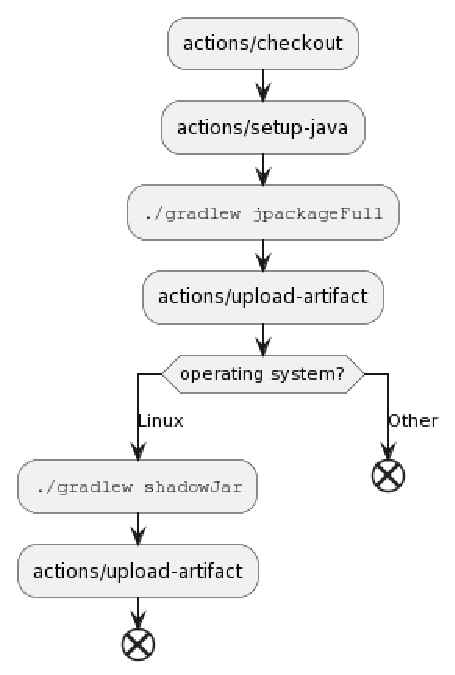
\includegraphics[width=.5\linewidth]{figures/generate-packages-job.pdf}
	\caption{Diagramma dell'attività del job incaricato a generare gli artefatti}
	\label{fig:generate-packages-job}
\end{figure}

Il job, raffigurato nella figura \ref{fig:generate-packages-job}, richiede solamente l'esecuzione di \texttt{select\--java\--version} necessaria ad impostare l'ambiente java nel runner. Una volta prodotti i pacchetti, questi saranno presi in carico dai successivi job per verificare il loro corretto funzionamento.

\subsection{Il processo di rilascio}

Come esposto nella sezione \ref{sec:release-limitation}, l'aggiornamento richiesto per il rilascio del software incontra limitazioni dettate dall'impostazione della pipeline, in particolare le possibilità di sviluppo sono limitate all'utilizzo di script o comandi da shell utilizzando un runner operante Linux.

Per abilitare la pubblicazione sull'Arch User Repository, è stato introdotto uno script bash nel progetto, accessibile facilmente dal comando del plugin adibito al rilascio. Lo script gestisce l'intera operazione nei seguenti passaggi: (i) configura le impostazioni ssh necessarie per l'autenticazione e la comunicazione con il repository, (ii) clona il repository corrente e imposta le credenziali del maintainer, (iii) sostituisce il PKGBUILD con quello nuovo, e infine (iv) crea il commit e lo pubblica nel repository, completando così l'aggiornamento del pacchetto. Le informazioni richieste sono configurate come parametri e fornite direttamente nell'esecuzione; tuttavia, i valori sono privati e non devono essere accessibili al pubblico. Mediante l'utilizzo dei \textit{secrets}, GitHub consente al maintainer del progetto di configurare variabili private accessibili nella sintassi YAML di GitHub Actions utilizzando il contesto omonimo secrets. In questo modo, i valori non sono leggibili da chi visualizza il codice sorgente del progetto.

\begin{figure}[htb]
	\centering
	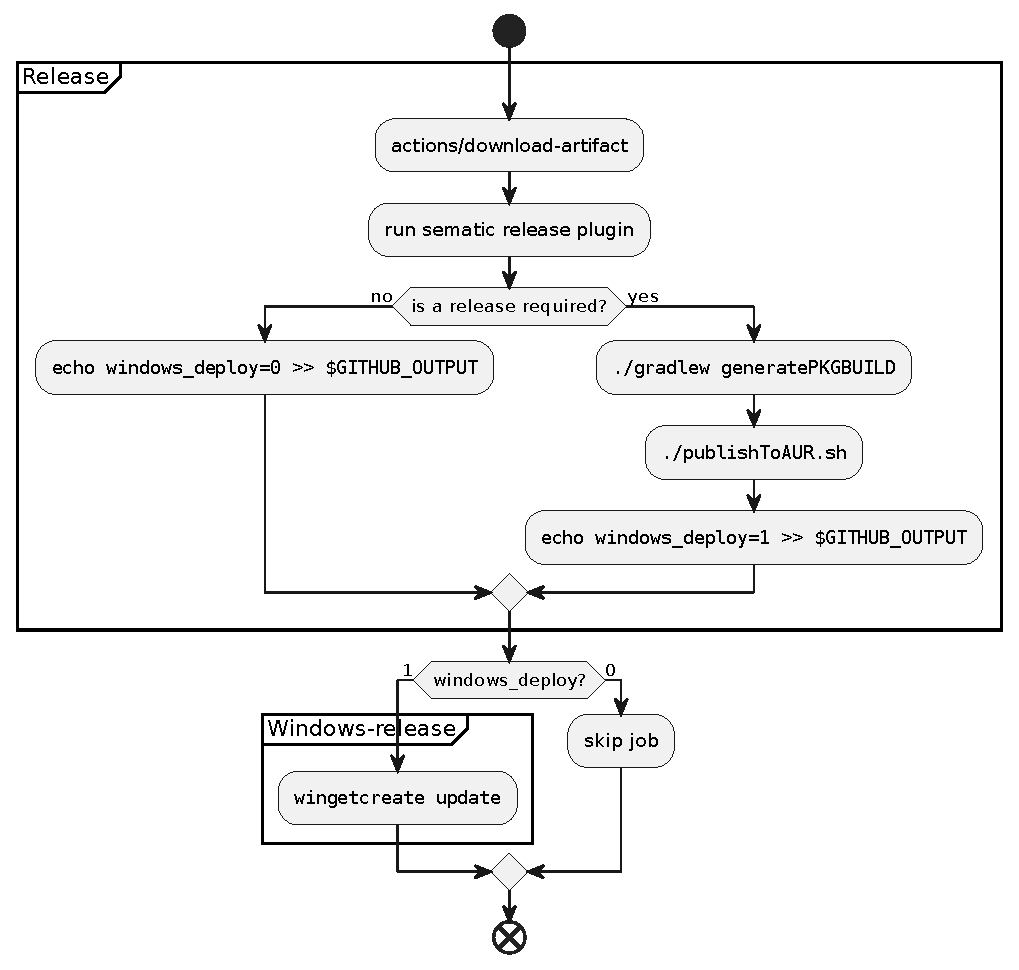
\includegraphics[width=.85\linewidth]{figures/release-flow.pdf}
	\caption{Diagramma dell'attività raffigurante il processo di rilascio su AUR e Winget}
	\label{fig:release-flow}
\end{figure}

Il processo di pubblicazione all'interno dei repository di winget richiede l'utilizzo di un runner Windows. In considerazione dei limiti e della necessità di non modificare la struttura della pipeline, è stato introdotto un job Windows complementare al rilascio. La sua esecuzione, tuttavia, deve dipendere dal plugin, il quale determina se il rilascio di una nuova versione è necessario. Nell'ottica di creare una relazione di dipendenza, il comando di pubblicazione del plugin: (i) imposta una variabile d'ambiente flag che stabilisce se il rilascio è stato eseguito, (ii) successivamente il suo valore è fornito in output mediante \texttt{\$GITHUB\_OUTPUT}, cosicché (iii) il job Windows accessorio determini se deve essere eseguito o saltato. Una rappresentazione semplificata dei due job è illustrata in una figura \ref{fig:release-flow}. Il ramo decisionale a destra descrive le azioni eseguite nel momento in cui è richiesto il rilascio di una nuova versione. La prima fase si occupa di generare il file PKGBUILD ed eseguire lo script riservato al repository AUR, mentre in un secondo momento il job complementare utilizza \texttt{wingetcreate} per procedere all'aggiornamento riguardante il package manager di Microsoft.

\subsection{Test dei processi}

Ogni processo aggiuntivo richiede lo sviluppo di un test apposito. Il fallimento di un qualsiasi test deve bloccare l'esecuzione della pipeline, cosicché si garantisce un processo di rilascio stabile e funzionante. Questa proprietà si ottiene attraverso lo sviluppo di verifiche di validità dei pacchetti e controlli riguardo la conformità dei meta-dati.

La verifica dei pacchetti richiede l'utilizzo di programmi specifici i quali dipendono dalla tipologia di pacchetto che si vuole analizzare. Utilizzando il build system ed integrando un task specifico \texttt{testJpackageOutput} si collassa la definizione di molteplici job all'interno di un job unico, il quale utilizzando la strategia a matrice definita precedentemente, permette la definizione di un solo insieme di attività poi distribuito su più runner con sistemi operativi differenti. Le procedure di installazione si trovano all'interno del task, il quale conosce il sistema operativo sottostante, dunque estrae i pacchetti relativi alla sua piattaforma e controlla la presenza dei file necessari all'utilizzo dell'applicazione. Il task estende la tipologia \texttt{Exec} fornita da Gradle che permette l'esecuzione di comandi nella shell del sistema operativo, in primo luogo configura il comando adibito ad installare il pacchetto a seconda della piattaforma su cui sta eseguendo (il blocco \texttt{doFirst} descritto nel listato \ref{lst:do-first-task}) ed infine una volta estratti utilizza le API di Kotlin per controllare il filesystem e quindi le cartelle generate durante l'installazione (il blocco \texttt{doLast}).

\lstinputlisting[float=htb,language=Kotlin,label={lst:do-first-task}, caption={Estrazione dei pacchetti utilizzando la tipologia di task \texttt{Exec}}, captionpos=b]{listings/task-package-extraction.kt}

Inizialmente il task era posto come dipendente dall'esecuzione di jpackage, in modo che l'esecuzione del test garantisse la presenza dei pacchetti. Questo comportamento tuttavia costringe la generazione dei pacchetti ogniqualvolta si voglia eseguire la verifica. Ciò accade perché il task fornitoci dal plugin \texttt{jpackage-gradle-plugin} non dichiara alcun \textit{output}, quindi Gradle non consente di utilizzare la funzionalità della \textit{build incrementale}. In altre parole, il build system non conosce l'output del task generatore e in caso i pacchetti siano già presenti, come accade nella pipeline perché generati da job precedenti, esso riesegue la generazione sovrascrivendo gli ultimi. La rimozione della dipendenza garantisce un incremento delle prestazioni, permettendo di dividere le attività in due unità di esecuzione differenti. Il costo è una minor chiarezza nell'utilizzo manuale del task, in quanto l'esecuzione del task di verifica senza previa generazione fallirà per l'assenza dei pacchetti. Siccome il test è sviluppato principalmente per l'utilizzo all'interno di pipeline, questa limitazione non genera particolari problematiche; generalmente gli sviluppatori non eseguiranno il task sulla propria macchina, e in caso fosse necessario è sufficiente indicare l'esecuzione del task generatore assieme a quello di verifica.

\section{Valutazione ed ottimizzazione}

L'implementazione descritta soddisfa i requisiti funzionali posti durante l'analisi. Lo sviluppo di nuovi processi all'interno del build system hanno consentito la pacchettizzazione del software per le piattaforme richieste mediante uno strumento esterno, jpackage. Funzionalità fornite da quest'ultimo hanno inoltre permesso una personalizzazione più approfondita dei pacchetti generati, permettendo l'esecuzione di comandi post-installazione e di conseguenza eliminando la necessità di configurazione da parte dell'utente finale. L'integrazione dei processi e delle relative verifiche all'interno della pipeline ha dato luce ad un flusso di continouous delivery completo, capace di rispondere alle esigenze dettate dalla filosofia DevOps.

Lo sviluppo della pipeline ha richiesto diverse revisioni prima di ottenere il risultato finale voluto. Il flusso di integrazione e distribuzione continua per sua natura è innescato continuamente ed è perciò fondamentale sfruttare le funzionalità fornite dall'API di Actions per ottimizzare la sua esecuzione. Per ottenere l'ottimizzazione desiderata esistono diverse accortezze nella configurazione dei workflow capaci di registrare incrementi prestazionali contenuti, ma che nel lungo periodo impattano positivamente lo sviluppo del progetto. Le principali ottimizzazioni utilizzate sono elencate di seguito:
\begin{itemize}
	\item \textbf{Fail-fast}: questa ottimizzazione si applica ai flussi di lavoro che definiscono una strategia a matrice. Se il fail-fast è abilitato, la piattaforma annullerà tutti i compiti in corso e in coda nella matrice non appena uno qualsiasi dei compiti in essa fallisce.
	\item \textbf{Concurrency group}: consente di inserire job all'interno di gruppi, identificati da una chiave, nella quale un solo job per volta viene eseguito. Normalmente Actions permette l'esecuzione dello stesso workflow, job e step parallelamente, ciò significa che la pubblicazione di diversi commit rapidamente  innesca l'esecuzione di più flussi paralleli. Se il flag \texttt{cancel-in-progress} è attivo e durante l'esecuzione di un job un altro componente dello stesso gruppo viene inserito in coda, quest'ultimo prende il posto ed elimina il job corrente.
	\item \textbf{Artefatti}: l'utilizzo delle action \textit{upload-artifact} e \textit{download-artifact} consentono di distribuire gli artefatti tra i job dei workflow. In generale, l'approccio preferibile è di stabilire dei job assemblatori che generano e forniscono gli artefatti a successivi job di test o rilascio. Il caricamento di file anche di notevoli dimensioni è estremamente più conveniente rispetto alla rigenerazione; file di dimensioni dell'ordine delle centinaia di megabyte sono processati in poche decine di secondi.
	\item \textbf{Timeout}: invece di fare affidamento sul timeout predefinito dei compiti, che è di 360 minuti (6 ore), i flussi di lavoro possono impostare esplicitamente un timeout personalizzato. L'opzione risulta efficace per interrompere i flussi di lavoro che si protraggono inutilmente a lungo, il che può essere particolarmente utile per evitare che i contributori, tramite pull request, inneschino flussi di lavoro prolungati.
	\item \textbf{Build system}: esso, nel caso specifico di Gradle, introduce un overhead dettato dalla necessità ad ogni esecuzione di effettuare le fasi di inizializzazione e configurazione. Sebbene implementi tecniche di ottimizzazione, l'utilizzo di Gradle, in particolare nei progetti di grandi dimensioni, può incrementare il tempo di esecuzione di un job di diversi minuti.
\end{itemize}

Si propone dunque un'analisi di quattro differenti versioni di pipeline sviluppate per Alchemist. La prima (\textit{a}) rappresenta il processo di integrazione e distribuzione continua utilizzato prima dell'intervento del progetto descritto in questo elaborato. Ciò ci consente di misurare il risultato ottenuto con le successive versioni in relazione al requisito non funzionale prestazionale introdotto in fase di analisi. La seconda (\textit{b}) descrive una struttura a job paralleli, la quale utilizza il build system sia per generare che per testare gli artefatti. La terza (\textit{c}) versione utilizza una configurazione sequenziale con distribuzione degli artefatti mediante le azioni di \texttt{upload/download-artifact}, mentre la quarta (\textit{d}), ed ultima versione, utilizza una configurazione prevalentemente sequenziale con caricamento degli artefatti, ma privata dell'utilizzo del build system nei job adibiti ai test. I tempi presi in esame sono ottenuti mediante la media aritmetica di dieci differenti esecuzioni dei flussi: l'\textit{execution time} indica il tempo di esecuzione del flusso nel suo complesso, mentre la \textit{total execution time} fa riferimento alla somma dei tempi di esecuzione di tutti i job all'interno della pipeline. Le quattro istanze prese in esame coinvolgono il normale flusso di integrazione e quindi non integrano l'esecuzione del job di rilascio.

\begin{figure}[htb]
	\centering
	\begin{tikzpicture}
		\begin{axis}[
			ybar,
            width=12cm,
			height=8cm,
			bar width=15,
			ylabel={ Time (h) },
			symbolic x coords={a, b, c, d},
			xtick=data,
			xlabel={Version},
			legend style={at={(0.5,-0.2)},
				anchor=north,legend columns=-1},
			]
			
			\addplot[blue!50!cyan,fill=blue!50!cyan] coordinates {(a, 0.81) (b, 0.77) (c, 1.12) (d, 0.74)};
			\addplot[red!70!orange,fill=red!70!orange] coordinates {(a, 2.12) (b, 2.55) (c, 3.11) (d, 2.78)};
			
            % Draw horizontal lines
			\legend{Execution Time, Total Execution Time}
		\end{axis}
	\end{tikzpicture}
	\caption{Grafico illustrante i tempi di esecuzione delle quattro differenti versioni di pipeline implementate}
	\label{fig:histogram}
\end{figure}
 
Innanzitutto, i risultati confermano un ottimo riscontro in relazione al requisito non funzionale, in particolare le due versioni \textit{b} e \textit{d} offrono prestazioni comparabili e contemporaneamente funzionalità aggiuntive rispetto la prima versione. L'utilizzo del build system peggiora le prestazioni, in quanto la quarta versione privata del suo utilizzo offre un miglioramento sostanziale rispetto la terza, la quale utilizza una configurazione similarmente sequenziale. La seconda versione (\textit{b}) ottiene risultati comparabili alla quarta (\textit{d}), nonostante non utilizzi il caricamento e scaricamento degli artefatti. Questo è dovuto alla mancanza del job incaricato al rilascio all'interno dei flussi analizzati. Mentre la versione \textit{d} ottiene gli artefatti da job assemblatori eseguiti precedentemente, la versione \textit{b} li genera nuovamente prima del loro rilascio. Di conseguenza, lo stesso test condotto su esecuzioni del flusso completo avrebbe mostrato un netto vantaggio della quarta versione rispetto alle altre prese in considerazione.

Dall'analisi dei dati risulta evidente come l'interazione con il build system, in particolare Gradle, prolunga l'esecuzione dei task per via delle fasi di inizializzazione dello strumento. L'utilizzo di un task, \texttt{testJpackageOutput}, per verificare la validità dei pacchetti, è risultato quindi controproducente. Sebbene quest'ultimo permetta una configurazione semplificata nel workflow, l'utilizzo di comandi shell è maggiormente indicato per svolgere semplici azioni che non richiedono particolari dipendenze.